\documentclass[letter]{article}
\usepackage[hmargin=0.5cm,vmargin=1.0cm,bindingoffset=0.0cm]{geometry}
\usepackage{amssymb}
\usepackage{amsmath}
\usepackage[letterspace=150]{microtype}
\usepackage{array}
\usepackage{wrapfig,lipsum,graphicx}
\usepackage[utf8]{inputenc}
\usepackage[T1]{fontenc}
\usepackage{lmodern}
\pagestyle{empty}
\parskip = 1.0 cm
\parindent = 0.0 cm

\newcommand\blank{\underline{\hspace{2cm}}} % Gives a blank 
\newcounter{prob} % A new counter for current problem number
\setcounter{prob}{1} % Start the counter at the value 1
\newcommand\itm{
\fbox{\textbf{\theprob}} \refstepcounter{prob}
} % Calls problem number
\newcommand{\problem}[1]{\makebox[0.5cm]{\itm}   
  \begin{minipage}[t]{\textwidth-0.5cm} #1 \end{minipage} 
}
\newcommand\divi[2]{
#2 \: \begin{array}{|l}
\hline #1
\end{array}
}

\newcommand\mult[2]{
$\begin{array}{rr} 
 & #1 \\ 
 \times & #2 \\ \hline 
 \end{array}$}
 
\newcommand\addi[2]{
  $\begin{array}{rr} 
   &  #1 \\ 
    + & #2 \\ \hline 
  \end{array}$}

\newcommand\subt[2]{
  $\begin{array}{rr}
    & #1 \\ 
    - & #2 \\ \hline
  \end{array}$}
\begin{document}
\setlength{\extrarowheight}{0.12cm}
\renewcommand\addi[2]{
\hspace*{5mm}\begin{tabular}{rr} \vspace{-2mm}
 & #1 \\
 $ + $ & #2 \\ \hline \vspace*{4.0mm}
 \end{tabular}}
\renewcommand\subt[2]{
\hspace*{5mm}\begin{tabular}{rr} \vspace{-2mm}
 & #1 \\
 $ - $ & #2 \\ \hline \vspace*{4.0mm}
 \end{tabular}}
\renewcommand\mult[2]{
\hspace*{5mm}\begin{tabular}{rr} \vspace{-2mm}
 & #1 \\
 $ \times $ & #2 \\ \hline \vspace*{4.0mm}
 \end{tabular}}

 

\begin{center} 
  \textsc{Arithmetic Worksheet}
\end{center} 


\begin{wrapfigure}[8]{c}{2cm}
  \centering
  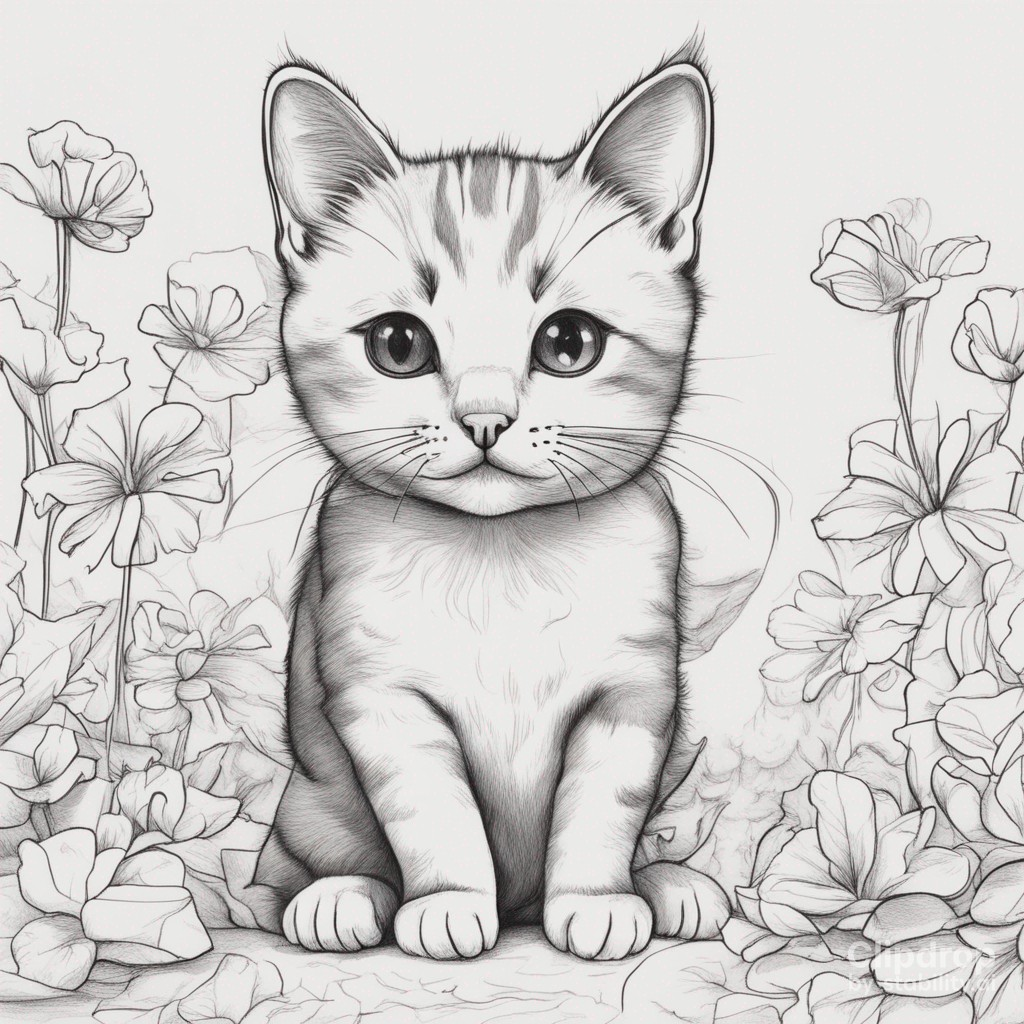
\includegraphics[width=\linewidth]{Ryan.jpg}
\end{wrapfigure}

        \begin{Huge}
Date:\underline{\hspace*{6cm}} \hfill
Name:\underline{\hspace*{6cm}}
\lsstyle



$$
\begin{array}{cccc}
\mult{12}{6} & \addi{21736}{724} & \mult{3}{12} & \addi{158}{4056}\\
\subt{852}{428} & \addi{406}{6433} & \divi{82}{22} & \divi{95}{5}\\
\subt{7498}{508} & \subt{721}{36} & \subt{2725}{27} & \divi{22}{5}\\
\divi{123}{22} & \divi{51}{19} & \subt{161}{125} & \addi{92}{92}\\
\addi{49921}{5784} & \addi{6796}{993} & \mult{11}{9} & \subt{66}{36}\\
\end{array}
$$
\end{Huge}
\end{document}
